\chapter{Implementation}
\label{impl}
The implementation chapter covers the technologies, techniques and patterns applied to this project.  Many of the contents were encountered were encountered during a summer placement at a technology company in Glasgow between levels 3 and 4.  

\section{Technologies Used and Discipline Applied}
This section examines the technologies used in the implementation of the project and the discipline that was adhered to during development.

\subsection{Microsoft .NET Framework}
The Microsoft .\gls{net} framework is a platform for development, deployment and running of web services and applications \cite{whatIsDotNet}.  It provides a \gls{clr}, similar to the \gls{jvm} in Java.  This project took advantage of \gls{asp}.\gls{net} \gls{mvc} 2.  

Microsoft's .\gls{net} framework was used as a result of encountering the technology during the summer placement.  The developer saw the opportunity of learning more about and working with the framework when the project was successfully assigned to him.  Given that one of the aims of the summer placement was to learn .\gls{net} development, and that this aim was not completely achieved \cite{summerPlacementReport}, the developer chose to maximise exposure to the technology by working with it for the duration of the project, and by adding the aim of learning the framework to the project goals.  It may appear that the choice of this framework was a short-sighted decision, but there are many other benefits to using this technology, including:
\begin{enumerate}
	\item There is an active developer community on the web\footnote{The community's forums can be found at \url{http://www.asp.net/community} and a large proportion of active users of the Stack Overflow community focus on \cs{} and .\gls{net} topics --- 3 of the top 8 tags are directly related to the project's domain --- \url{http://stackoverflow.com/tags} (by observation)}, so issues pertaining to development using the framework can be solved by turning to this well-grounded knowledge base;
	\item The \gls{mvc} aspect of the project, if strictly adhered to by the developer, provides great separation of concerns between the place that information is stored, manipulated and viewed;
	\item The framework allows for portability to other client machines with very little in the way of model adjustment. For example, if a requirement for a mobile or tablet application developed, it would simply be a case of adding the functionality for that device, rather than having to reimplement the model for a particular piece of hardware.
	\item Applications can be deployed, with some adjustments, on Linux machines using the Mono (open source) software platform \revisit - awaiting help from Gregg
\end{enumerate}

\glsreset{oo}
\subsection{\cs}
\label{csharpDiscussion}
\cs{} is an \gls{oo}, garbage-collected programming language which has roots in the C family of languages.  It is a standardised language (ECMA-334 and ISO/IEC 23270) with compilers available for unix based systems (using the `Mono' compiler) and Windows systems (using Microsoft's \cs{} compiler for the .\gls{net} Framework) operating systems, which both conform to the ECMA and ISO/IEC standards \cite{monoStandardised} \cite{csPL}.

\cs{} was used over the other .\gls{net} languages (of which there are at least 30) \cite{csUnleashed} because the developer wanted to become familiar with the language having encountered it and used it while on summer placement.

\subsection{NHibernate and Fluent NHibernate}
\label{nhibernate}
NHibernate is a port of the Hibernate object/relational mapper to the .\gls{net} framework. In essence, it provides mapping from objects to relational tables, which allows a developer to concentrate on functionality and usability rather than spending time writing \gls{sql} scripts. Queries are generated by NHibernate middleware and passed to the database which, after execution, accumulates any results into objects directly manipulable by \cs{} code. 

An example of how this technology helps and works is described presently: Let's assume that a series of valid entries have been created in the database and that a user has issued a request to view the details for one of them, with the \gls{id} 3.  Sample code to fetch the publication associated with this Id and return it as a usable object is shown in figure \ref{fig:fetchPubCode}.

\begin{figure}
	\begin{center}
			\lstset{language=CSharp} 
			\begin{lstlisting}
	public static Publication GetPublication(int givenID)
	{
	    // Get an NHibernate session with the database
	    ISession ses = GetSession(); 
	
	   	// LINQ query used to construct SQL query in middleware
	    IQueryable res = from pubs in ses.Linq<Publication>()
	                     where pubs.Id == givenId
	                     select pubs;
	                        
	    // pull the first item from 'res' 
	    Publication thePublication = res.First();
	    
	    return thePublication;
	}
			\end{lstlisting}
		\caption{Code to fetch a Publication by ID}
		\label{fig:fetchPubCode}
	\end{center}
\end{figure}

The code in figure \ref{fig:fetchPubCode} returns the publication for manipulation in code; recording changes made to the entry after manipulation (or saving an entry for the first time) is very simple, as shown in figure \ref{fig:storePublication}.

\begin{figure}
	\begin{center}
			\lstset{language=CSharp} 
			\begin{lstlisting}
	// saves the item for the first time if it does not yet exist
	// or updates the entry if it already exists (pubVar is of type 'Publication')
	pubVar.SaveOrUpdateInDatabase();
			\end{lstlisting}
		\caption{Code to store a publication after creation or modification}
		\label{fig:storePublication}
	\end{center}
\end{figure}

The NHibernate software itself is highly valuable in terms of time-saving potential and has been used across thousands of successful projects \cite{NhUse}.  The only issue with using it in its raw form is that mappings from the project's classes to relational entities have to be written in \gls{xml}, a language prone to errors often left unnoticed until runtime.  A better solution is to use the \gls{fnh} extension, which provides developers with the ability to map the classes in code.  The major benefit of this scheme, aside from compile-time error checking, is that all code using is strongly-typed; combine this with the powerful \gls{msvs} \gls{ide}, and implementation for the data model can be quite rapid --- particularly when in the hands of an experienced developer.

Another reason for using this technology was that it was used within the summer placement, but it was not encountered or worked with to any great extent.  The developer wanted to expand his knowledge in the technology in both breadth and depth by adopting these technologies within the project.

There was a risk, when employing this technology, that unfamiliarity would lead to hindrance rather than benefit by employing it.  Before automatic generation of database scripts for interactions can take place, \gls{fnh} has to be instructed what to map and how to map it.  This was not something that the developer had encountered before; the risk was that learning how to map the classes to entities correctly would take too much time and have an impact on the progress of the project.  To mitigate the impact of the risk, a deadline was agreed between the developer and the supervisor: if, by the final day of term in semester 1, the mappings were not working correctly, then NHibernate as a data solution would be abandoned and standard \gls{sql} queries would be used.  As it turned out, the mappings were finalised on the afternoon of the deadline, so NHibernate use went ahead.  The aforementioned benefits of NHibernate were noticed during development, and some experience was gained in the implementation and use of object/relational mapping in practice.

As the project progressed and the developer became more familiar with \gls{fnh}, it was discovered that the extension can `Automap' classes: something that would have been quite helpful in the lead up to the end of semester 1 NHibernate risk-mitigation deadline.
The code to take advantage of the automap feature is listed in figure~\ref{fig:fnhCode}:

\revisit

\begin{figure}
	\begin{center}
			\lstset{language=CSharp} 
			\begin{lstlisting}
// get relevant code!
			\end{lstlisting}
		\caption{Code to take advantage of Fluent NHibernate's Automapping facility}
		\label{fig:fnhCode}
	\end{center}
\end{figure}

\section{Development Environment}
\label{devEnv}
Most of the development took place on the developer's laptop, a MacBook Pro dual-booted with Windows 7 Professional.  Some development took place on a second developer machine when the laptop was unavailable.

The main development environment was Microsoft's Visual Studio Professional 2010 (\gls{msvs}), provided by the School's \gls{msdnaa} agreement.  This was the same environment used while on summer placement, so the developer was familiar with the tools in the \gls{ide}.

The database product used was \gls{msss} 2008 Developer Edition, again provided by the School's \gls{msdnaa} agreement. The management suite included with the product was again used while on summer placement, and the developer was familiar with the tools in the program.

ReSharper is a productivity plug-in for \gls{msvs}.  It provides code inspections, code analysis, one-click unit test runs, project-level refactorings and many more assistive features. A licence for the product was bought during the summer placement and was used extensively throughout the development of the software article.

Python IDLE and Notepad++ were used to manipulate code quickly and effectively: Python IDLE for its scripting functionality and Notepad++ for its macro capabilities and excellent search and replace by regular expression function.

TortoiseSVN and AnkhSVN were both used as discussed in section \ref{svn}.

\section{Code Reuse}
\label{codeReuse}
Code reuse from previous projects during this product's development was intended to be maximised, as laid out in section \ref{columbia}.  The benefits of this include that time can be saved by reusing successful approaches and code that has been previously used (and therefore tested through use) is less likely to contain large flaws and bugs.

The only component that was reused from previous projects in the final deployment version was Mitesh's \bibtex{} file parser;  initially, the code was simply ported from Java to \cs, but as the project progressed, it became apparent that there was a rather important problem with it: the way that errors were dealt with was not user-friendly, which meant that errors could not be recovered from.  This risk emerged through use of the system and was not a problem identified at early stages of the project and had to be dealt with as it progressed.

The string libraries for \cs{} and Java do not match completely.  Some of the Java methods had to be implemented in \cs{} code to simplify the transition, namely:
\begin{enumerate}
	\item Java's String.equalsIgnoreCase() method does not have an equivalent in \cs, which was addressed by adding a class named `Compare' with the method implemented in \cs;
	\item Java's StringBuilder library was not a good match with \cs's StringBuilder library; the subString, indexOf and lastIndexOf methods do not exist, and were as a result implemented as static methods in \cs{} in the parser class.
\end{enumerate}

The parser does not deal with some \bibtex{} format features, specifically:
\begin{enumerate}
	\item the `\#' character (used as a concatenation operator) is future work for the parser;
	\item it is not currently possible to use `@string' variables;
	\item `@comment' tags will not work if it is intended to `comment-out' an entry from a file.
\end{enumerate}
	


\section{Data Model}
\label{dataModel}
The design of the data model is discussed heavily in chapter \ref{design} and a \gls{uml} model of the final approach taken can be found in figure~\ref{fig:ChallengerClassDiagram}.

The data model is implemented in two parts: firstly, the class model of the Publication structure; and secondly through the use of NHibernate (see section \ref{nhibernate}) for storage.


Discuss implementation of data model, implementation of database persistence. centralised persistence information - single section of code + benefits.
The data model, as mentioned in section \ref{nhibernate}, is implemented using NHibernate.  
Discuss fields in publication table. Mention creation/modification/deletion times and what they are used for
ID field vs cite key
owner


An item is marked as deleted if its DeletionTime has a non-null value.  This is a standard adopted throughout the system: any entry which has a null value for its DeletionTime is regarded as an active entry in the system; conversely, an entry which is marked as deleted is subject to the expiry time of 60 seconds (a preliminary value used in the system), after which it may be deleted in the classic sense of the word.  This allows users to restore entries which have been deleted in case there has been a mistake in its removal.  All deleted entries  in the system can be viewed by accessing the `View Deleted Entries' option in the `View' section of the menu area.

\section{Search}
\label{searchCore}
The search is facilitated by the DataPersistence class, by way of the GetActivePublicationsMatching(searchString) method.  

\begin{enumerate}
	\item Firstly, the string is prepared for the database, to allow for wildcards;
	\item Secondly, the search is carried out across the database;
	\item Thirdly, results are collated to \cs's List type and returned for use by the calling method.
\end{enumerate}

Users search by strings, which can include the wildcards '*' for any sequence of characters and '?' for any single character.
This is facilitated by the method entitled \texttt{PrepareSqlString} in the \texttt{DataPersistence} class as shown in figure \ref{fig:SQLsearchEscape}.

\begin{figure}
	\begin{center}
			\lstset{language=CSharp} 
			\begin{lstlisting}
  private static string PrepareSqlString(string s)
  {
      // escapes SQL wildcards and inserts SQL wildcards in
      // place of characters * and ?
      
      // check for % signs and replace with \%
      s = Regex.Replace(s, "%", "\\%");
      // Check for * signs and replace with %
      s = Regex.Replace(s, "\\*", "%");
      // Check for _ signs and replace with \_
      s = Regex.Replace(s, "_", "\\_");
      // check for ? signs and replace with _
      s = Regex.Replace(s, "\\?", "_");
      return s;
  }
  		\end{lstlisting}
		\caption{Code to escape SQL wildcards and convert asterisks and question marks into SQL-query friendly strings}
		\label{fig:SQLsearchEscape}
	\end{center}
\end{figure}

The search is performed by the method in the DataPersistence class entitled GetActivePublicationsMatching(string s), which can be seen in figure \ref{fig:PerformSearch}.  This code snippet is a good example of how the strongly-typed, \gls{oo} queries (benefits of NHibernate mentioned in \ref{nhibernate}) are used effectively and efficiently.  They are written in \gls{linq}, a language which addresses the needs of developers by enabling support directly in the programming language \cite{csUnleashed}.

\begin{figure}
	\begin{center}
			\lstset{language=CSharp} 
			\begin{lstlisting}
	public static IList<Publication> GetActivePublicationsMatching(string s)
	{
	    // prepare the SQL string - escape SQL wildcards 
	    //         and replace * and ? characters
	    s = PrepareSqlString(s);
	    
	    // Get a session with the database
	    var currentSession = GetSession();
	
	    // Put together the search query in LINQ and execute it
	    var a = from pub in currentSession.Linq<Publication>()
	            where pub.DeletionTime == null &&
	                  (pub.CiteKey.Contains(s) ||
	                  pub.Address.Contains(s) ||
	                  pub.Annote.Contains(s) ||
	                  pub.Authors.Contains(s) ||
	                  pub.Booktitle.Contains(s) ||
	                  pub.Chapter.Contains(s) ||
	                  pub.Crossref.Contains(s) ||
	                  pub.Edition.Contains(s) ||
	                  pub.Editors.Contains(s) ||
	                  pub.Howpublished.Contains(s) ||
	                  pub.Institution.Contains(s) ||
	                  pub.Journal.Contains(s) ||
	                  pub.TheKey.Contains(s) ||
	                  pub.Month.Contains(s) ||
	                  pub.Note.Contains(s) ||
	                  pub.Number.Contains(s) ||
	                  pub.Organization.Contains(s) ||
	                  pub.Pages.Contains(s) ||
	                  pub.Publisher.Contains(s) ||
	                  pub.School.Contains(s) ||
	                  pub.Series.Contains(s) ||
	                  pub.Title.Contains(s) ||
	                  pub.Type.Contains(s) ||
	                  pub.Volume.Contains(s) ||
	                  pub.Year.Contains(s))
	            select pub;
	
	    // convert the results to a list and return them
	    return a.ToList();
	}  		
			\end{lstlisting}
		\caption{Code to perform a search}
		\label{fig:PerformSearch}
	\end{center}
\end{figure}

\section{Controller}
Home controller
Account Controller
Entry controller:
 - Same page for add and amend
 - discuss import
 - 
Discuss handling of requests


\section{Web Service}
The project has several areas which are performed by \gls{ajax} interactions with the system.  These interactions are handled by a web service entitled `SearchResults'. It was initially intended to handle only the instant search result collation; refactoring was attempted to rename the service to a more representative name, but there were too many issues with the name change, hence the slightly misleading name.

The instant search function is supported by a web service which accepts a search string, performs a search on the database by reusing the search method discussed in section~\ref{searchCore}, and returns the results in \gls{json} array, for the client-side code (\gls{js}) to deal with.  

Delete functionality and duplicate reduction functionality are both provided by \gls{ajax} requests by calls to the DeletePublication(int id) method of the web service.  It again reuses the DataPersistence class's method of the same name to mark an entry in the system as deleted, before returning the result to the client.

A deleted entry (see section~\ref{dataModel} for the model's definition of `deleted') is timestamped with the time of its deletion, which can be used to determine entries which have been deleted since a given time by comparing the given time with the deletion time. 

The web services provides a behind-the-scenes ability to find out what entries have been deleted since a given time.  This core code which performs the result accumulation is shown in figure \ref{fig:getDeletedPublicationsWS}; some of the code, particularly exception-handling clauses, is excluded here for brevity.

\begin{figure}
	\begin{center}
			\lstset{language=CSharp} 
			\begin{lstlisting}
  // Parse the given creation time into a DateTime object
  DateTime d = DateTime.Parse(pageCreationTime);

  // Get deleted entries into a list
  var pubs = (from publications in DataPersistence.GetSession().Linq<Publication>()
              select publications).ToList();
  pubs = pubs.Where(p => (p.DeletionTime.HasValue)).ToList();

  // create the list of results
  IList<int> result = new List<int>();
  foreach (Publication publication in pubs)
  {
      if (publication.DeletionTime != null)
          // if the deletion time is newer than DateTime d, add it to the return list.
          if (publication.DeletionTime.Value.CompareTo(d) > 0)
              result.Add(publication.Id);
  }

  return result;
			\end{lstlisting}
		\caption{Code to retrieve deleted entries since a given time}
		\label{fig:getDeletedPublicationsWS}
	\end{center}
\end{figure}

This approach is used to facilitate concurrent access by notification that items have been changed in the system.  

Similarly to the way deleted entries' times are tracked, the amendment and creation times of an entry is tracked by a field entitled `AmendmentTime' and `CreationTime' respectively.  A list of recently-amended or created entries can be accumulated by the same algorithm as for deleted entries.

The use of these web services in the concurrent access aspect of the system is discussed fully in section~\ref{concurrency}.

\section{View}
\glsreset{ui}
\subsection{Consistency}
The consistency sought in the design of the product (see section \ref{uiDesign}) of the site is a result of careful consideration of what should be consistent across all pages, as highlighted in figure \ref{fig:pageLayout}, which has certain features annotated numerically as follows:

\begin{figure}
	\begin{center}
		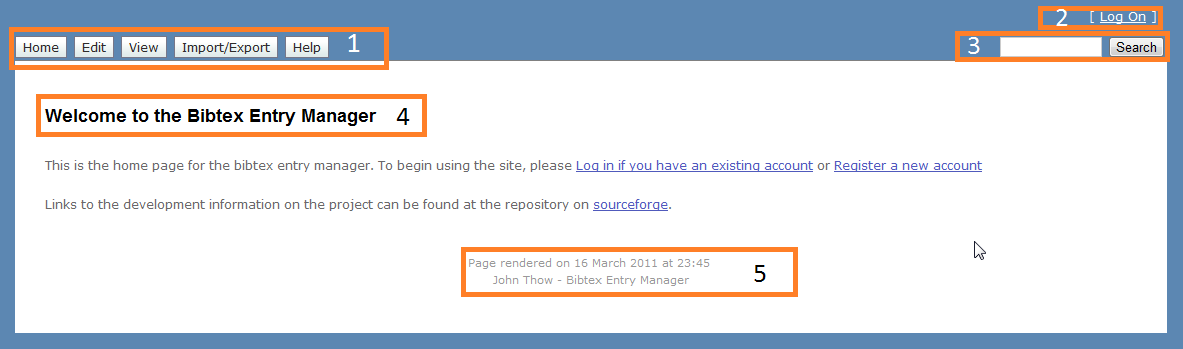
\includegraphics
			[scale=0.5]
			{images/PageLayout.png}
		\caption{Annotation of a page}
		\label{fig:pageLayout}
	\end{center}
\end{figure}

\begin{figure}
	\begin{center}
		
\includegraphics
			{images/LogOff.png}
		\caption{The log on area when a user is logged in (swapped out for area 2 in figure \ref{fig:pageLayout})}
		\label{fig:logOff}
	\end{center}
\end{figure}

\begin{enumerate}
	\item Firstly, there is a menu area which appears on every page within the site, with the same options at each appearance.  This gives the user a single point of reference to aid navigation of the website \revisit - cite someone
	\item The log on area appears in one of two forms across all pages of the application: a user is either browsing anonymously, or is logged in.  It is clear which of these two states the user's session is in thanks to the clear representation of the words `Log On' (depicted in figure \ref{fig:pageLayout}) and a welcome message with the current user's email address (as depicted in figure \ref{fig:logOff})
	\item After feedback from a user during the basic evaluation (see Chapter \ref{eval}) the interface was updated to include a search area on all pages.  The provision of this area allows a user to efficiently search the system's database for a string and, by making it a consistent feature, gives another concrete point of reference across all pages.
	\item Each and every page contains a bold header indicating the title of the page.  The presence of a title on each page gives a user another concrete and consistent place to glance in order to gain an insight into what they previously clicked on, as well as giving confirmation that their previous action was successful.
	\item The fifth item highlighted in this image provides some extra, arguably unnecessary information.  The main idea behind including this page render time area is to provide extra feedback: it lets a user know that page has finished loading, that it has been completed successfully and it reassures a user that the page is up to date.
\end{enumerate}

This consistency was implemented using a feature in \gls{asp}.\gls{net} called Master Pages.  As the name suggests, the developer creates a master page with the main layout of the website, within which sit containers which are filled by individual pages.  This approach centralises the code for the pages, the advantages and disadvantages of this are discussed in section \ref{codeReuse}. \revisit revisit fluency.

The colour choice of the interface was a decision which was postponed until later in the project, so that the bulk of the development work could be carried out before aesthetics were considered.  The colour scheme seen in the project is heavily based on the default style for projects created in \gls{msvs} 2010; it soon became apparent that the default style had many strong qualities that could be used 

\section{Concurrency}
\label{concurrency}
Possible approaches:\\
Pessimistic: Lock users out while one works on it \\
Optimistic: Allow all to view/delete/amend and notify when others have performed actions\\
No concurrency control, real-time updates instead

\section{Subversion}
\glsreset{svn}
\label{svn}
\gls{svn} is a centrally-stored version control system which records every change ever made to the files and directories in the file repository \cite{CFP04c1}.  It is useful to be able to centralise the code repository and to be able to synchronise different workstations with the most up to date version of code and documents, as well as allowing the logging and comparison of different versions of the code.  Each time information is updated in the repository, it is said to have a new revision -- a process also known as `committing' changes.  It was decided early in the project that a repository would be used to mitigate the risk of fire, flood, theft, and hard drive corruption by hosting the repository in a different physical location to the main work environment, the developer's laptop.  

\gls{svn} was used to control different versions of the code and to take snapshots of the project in the form of \gls{svntag}s \cite{CFP04c4}, as well as normal revisions.  It was originally hosted on the School of Computing Science network because it was accessible from outside the School's network of computers\footnote{access was facilitated by the School's \gls{ssh} gateway, \texttt{sibu.dcs.gla.ac.uk}}, because there was sufficient storage space provided by the School and it had no financial cost.  As part of the effort to ensure good software engineering practice, \gls{ci}\footnote{See Section \ref{continuousIntegration} for an explanation of what it is and why it was used} was to be used with the project, again after encountering it while on summer placement.  Unfortunately, there were problems in configuring the  \gls{ci}  software to access the \gls{svn} repository through the gateway; as a result of this, on the 16\^{th} of November 2010, the repository was moved to another free host, SourceForge, an open-source software project hosting provider.  Along with \gls{svn} repository hosting, SourceForge provides tools for management of software projects, including a bug tracking tool (see Section \ref{bugTracking}).  Crucially, the SourceForge repository was accessible by the \gls{ci} software, allowing the \gls{ci} process to take place.

The \gls{svn} client in most cases was TortoiseSVN, as development was to take place on a windows environment.  AnkhSVN, a secondary client, was also used as it integrated with the \gls{msvs} \gls{ide}. 

The change log from the \gls{svn} repository is included as an appendix\revisit; the repository can also be browsed on the SourceForge website at \url{http://bibman.svn.sourceforge.net/}

